\section{Compressed Operations}
\label{sec:ops}

Performing linear algebra operations---like matrix multiplications, element-wise operations,
and aggregations---on compressed matrices can improve memory-bandwidth requirements and cache utilization,
reduce the number of floating point operations, and preserve structural redundancy across chains of operations.
\name\ makes extensions for compressed matrix-matrix multiplications and compressed intermediates, which broaden its applicability.

\subsection{Design Principles and Notation}

As a basis for discussing compressed operations, we first establish necessary terminology, and summarize underlying design principles.

\textbf{Definitions and Scope:}
We define \emph{sparse-safe} operations as operations or aggregations that only need to process non-zero input cells.
For example, $\text{round}(\mat{X})$ is sparse-safe, while $\text{exp}(\mat{X})$ is sparse-unsafe because $\text{exp}(0) = 1$.
\emph{Special values} like NaN (not-a-number, with $\text{NaN} \cdot 0 = \text{NaN}$) are not supported compressed because they render sparse linear algebra invalid \cite{Sommer0ERH19}.

\textbf{Design Principles:}
Many of the \name \ operations share the following design principles. Compared to CLA, \name\ applies these principles to more operations and generalizes them with the goals of redundancy exploitation and minimizing total execution time.
\begin{itemize}
	\item \emph{Shared Index Structures:} For operations that only modify distinct values (e.g., $\mat{X} \cdot 7$), we perform dictionary-local operations and shallow-copy the index structures into the output.
	\item \emph{Memoized Tuple Frequencies:} Operations like $\text{sum}(\mat{X})$ aggregate the distinct tuples scaled by their frequencies. To avoid redundant computation, we memoize computed frequencies and retain them on shallow-copies of indexes. 
	\item \emph{Exploited Structural Redundancy:} While many sparse-unsafe operations can be executed on compressed matrices, they can require the materialization of zero, which often creates large unbalanced groups. Instead, in \name\, we exploit both sparsity and redundancy via the handling of default values, as well as preserve structural redundancy across operations.
	\item \emph{Soft References:} We keep useful but recomputable data structures (e.g., decompressed data, offset pointers to indexes, and tuple frequencies) on soft references. Any serialization or memory estimates do not include these cached objects.
\end{itemize}

\textbf{Notation:}
Finally, we need some additional notation.
An $n \times m$ uncompressed input matrix is compressed into a set of column groups $\mathcal{G}$, where $\card{\mathcal{G}}$ denotes the number
of column groups (with $\card{\mathcal{G}} \leq m$ without overlap), and $\mathcal{G}_i$ denotes the $i$-th column group.
A single column group $\mathcal{G}_i$ comprises $\card{\mathcal{G}_i}$ columns, a $d_i \times \card{\mathcal{G}_i}$ dictionary $\mat{D}_i$ with $d_i$ distinct tuples,
and an index structure $\mat{I}_i$. For matrix multiplications $\mat{A}\,\mathcal{G}$ or $\mathcal{G}\,\mat{B}$,
let $k$ denote the number of rows in \mat{A} and columns in \mat{B}, respectively.
Given a matrix or vector \mat{X}, $nnz(\mat{X})$ denotes its number of non-zeros and $nnd(\mat{X})$ denotes its number of non-default values
(equivalent to $nnz(\mat{X})$ if zero is the most frequent value).


\subsection{Matrix Multiplications}

CLA supports only matrix-vector and vector-matrix multiplications directly on compressed representations,
but emulates matrix-matrix multiplications via repeated slicing and matrix-vector multiplications.
This approach provides simplicity and reasonable performance, but looses performance as the size of the second matrix increases,
which is common in applications like multi-class classification, dimensionality reduction, and clustering.
Other previous work like TOC \cite{LiCZ00NP19} supports matrix-matrix multiplication but belongs to the class of grammar-compression.
In this section, we introduce simple yet impactful techniques for matrix-matrix multiplications on lightweight compressed matrices,
including special cases of compressed-compressed multiplication.

\textbf{Preaggregation:} A central technique of compressed matrix multiplications are different forms of pre-aggregation over the distinct tuples.
In \name, we vectorize such pre-aggregation for improved simplicity and performance.
For instance, Figure~\ref{fig:preagg} shows the intuition of pre-aggregation in left and right matrix multiplication on our running example.
First, for a left matrix multiplication $\mat{A}\,\mathcal{G}$ with an uncompressed vector \mat{A},
we initialize a zero vector $\mat{P}$, and accrue the entries of A according to indexes $\mat{I}_i$.
Subsequently, a simple uncompressed vector-matrix multiplication $\mat{P}\,\mat{D}_i$ of the pre-aggregates and the dictionary yields the overall result (for columns of the column group).
Instead of multiplying all entries with the same distinct value (or tuple in case of co-coding),
we simply distribute multiplication over addition.
Second, for a right matrix multiplication $\mathcal{G}\,\mat{B}$ with an uncompressed vector \mat{B} (subset relevant to the column group),
we first compute a matrix-vector multiplication of $\mat{D}_i\,\mat{B}$ to get the pre-aggregated vector $\mat{P}$, and subsequently add these pre-aggregated values to the output according to indexes $\mat{I}_i$. Interestingly, a similar pre-aggregation strategy is also applied as a general case for unnesting correlated subqueries \cite{0001K15}. Given this vectorized form and the storage of dictionaries as uncompressed matrices, we can directly apply cache-conscious uncompressed matrix multiplications for the general case of left- or right-hand-side uncompressed matrices with k rows or columns, respectively.

\begin{figure}[!t]
	\centering
	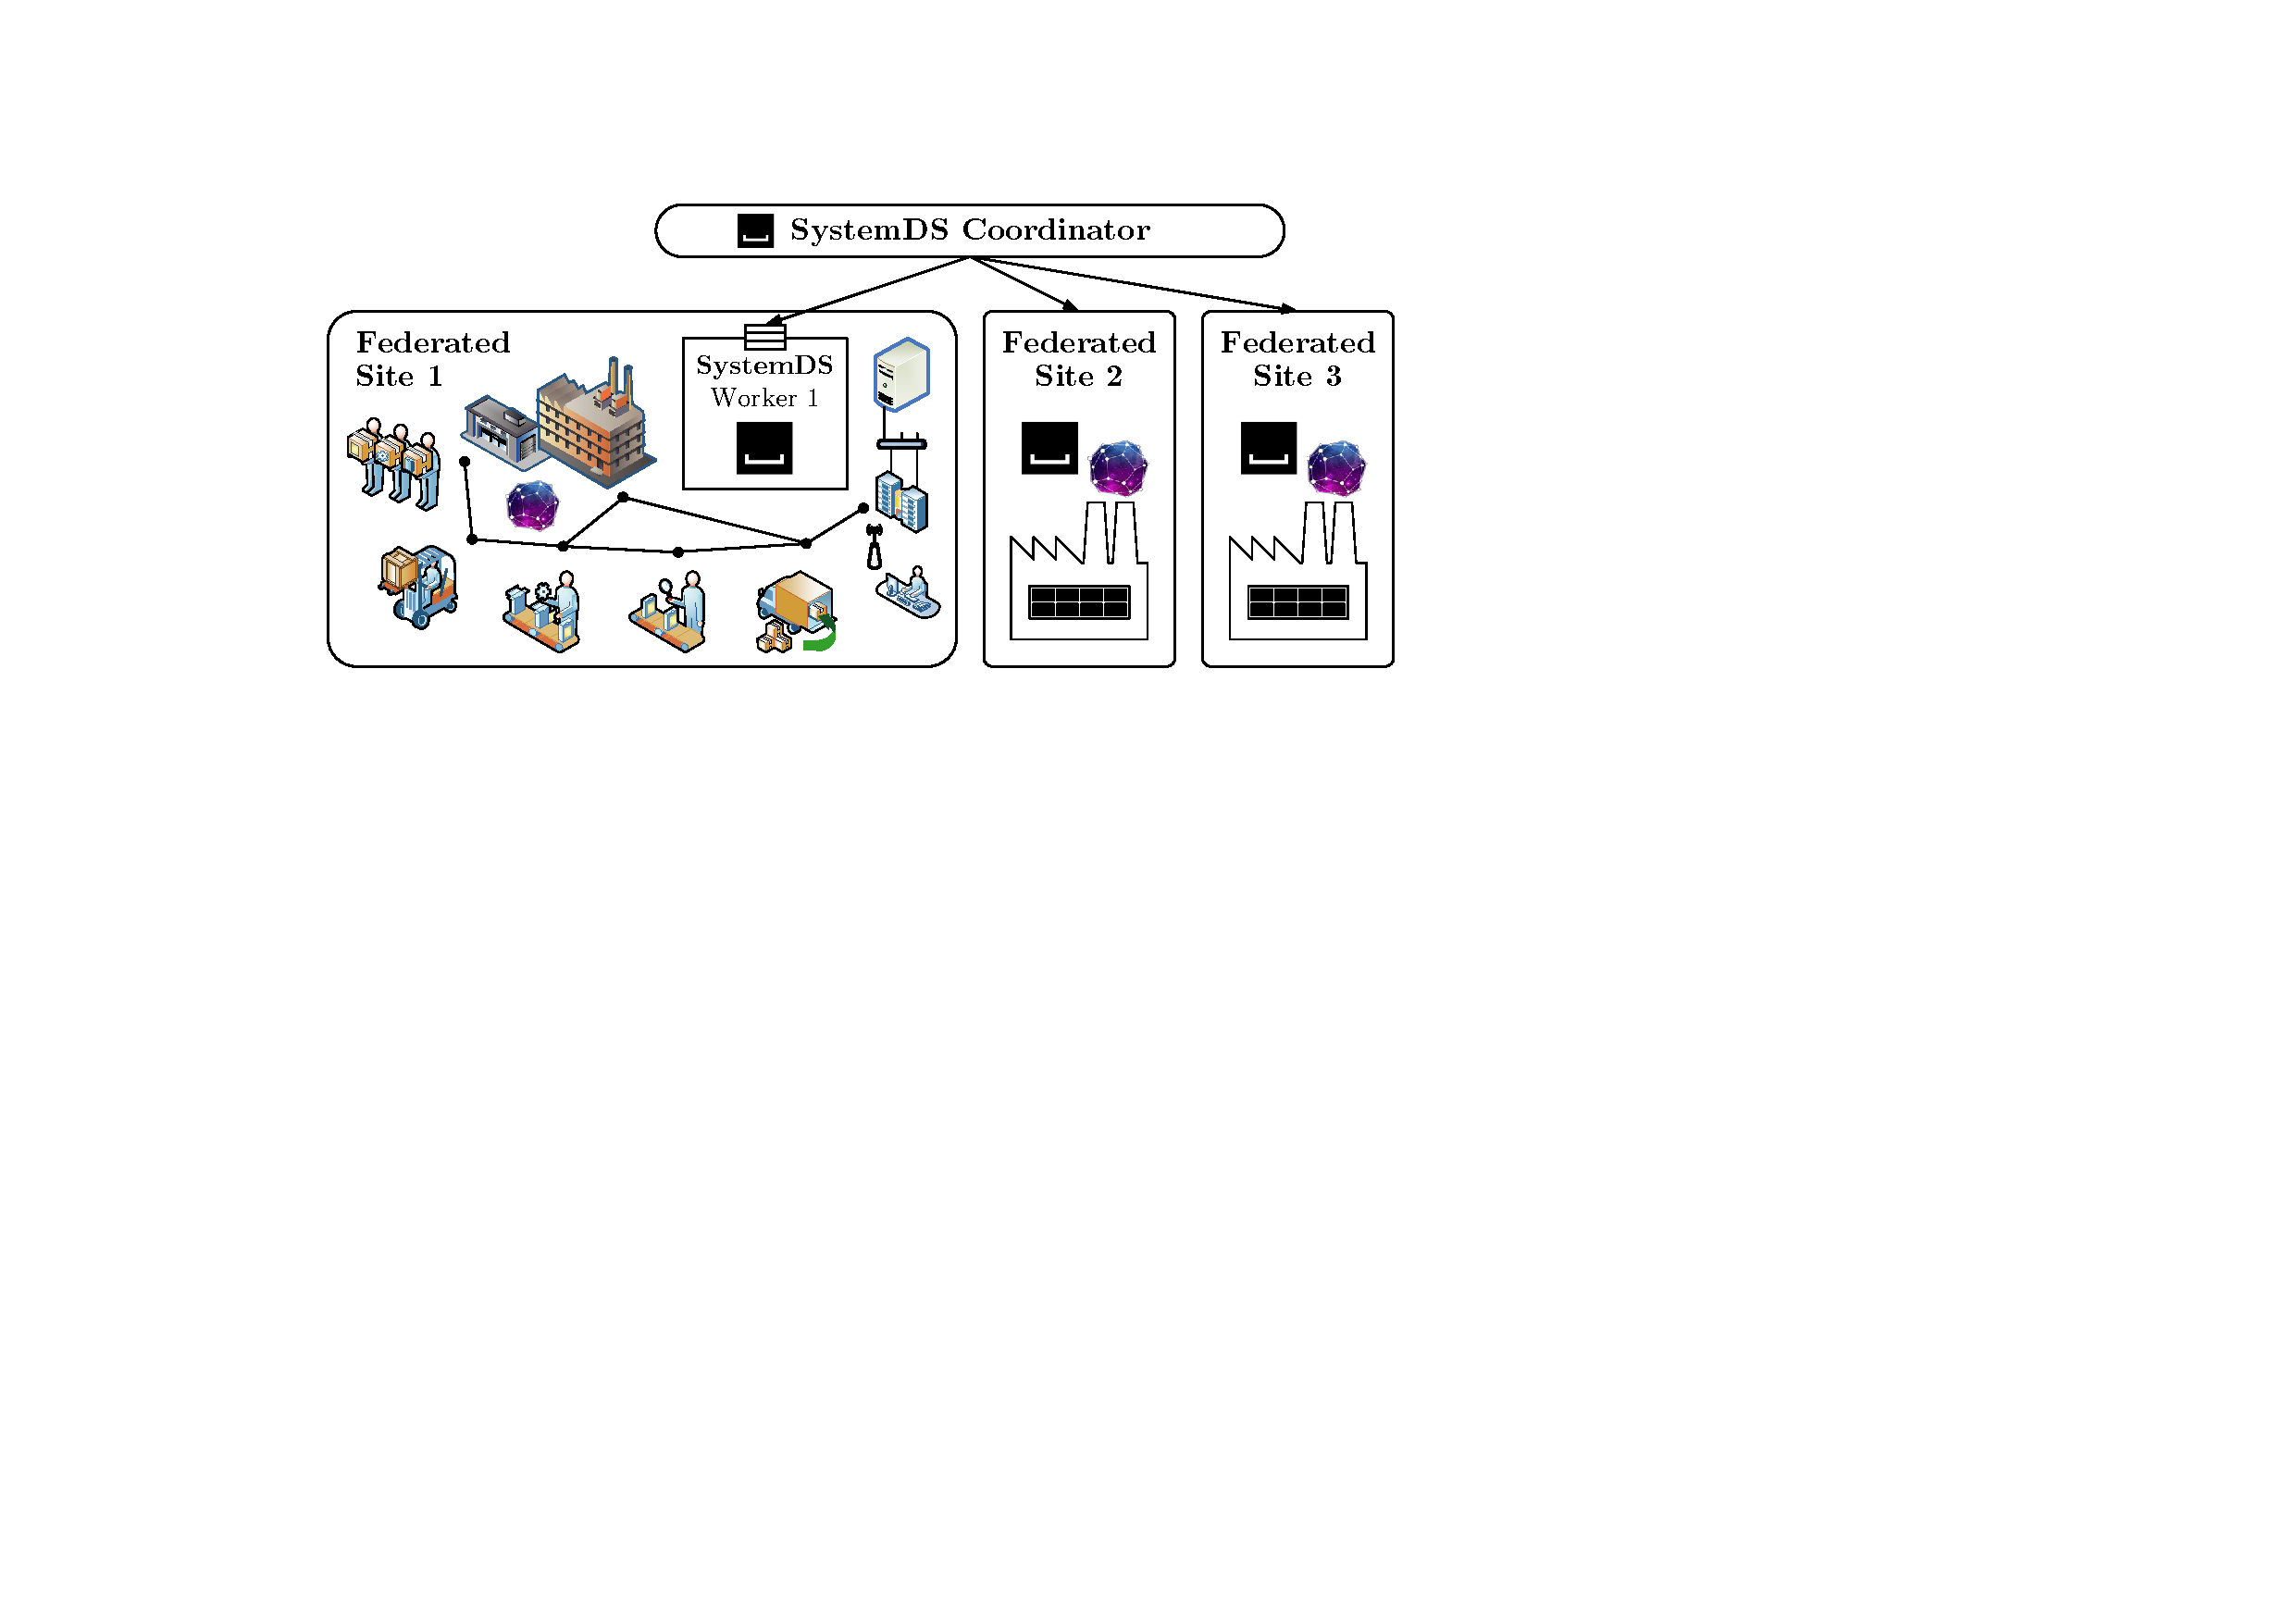
\includegraphics[width = 0.8\linewidth]{fig/fig04}
	\vspace{-0.25cm}
	\caption{\label{fig:preagg}Example Pre-aggregation in Compressed MatMult.}
	\Description{}
\end{figure}


% \begin{algorithm}
% 	\caption{LMM Algorithm}\label{alg:lmm}
% 	\Small
% 	\begin{algorithmic}
% 		\Require{$A$ , $G$} \Return{$R$}

% 		\State $(G^{m}, constRow) \gets Morph(G) $
% 		\State $P \gets allocatePreaggregate(|G^m|)$
% 		% \State $rowSums \gets rowSum(A) $
% 		\For{ $rb \gets 0$ to $nRow(A) / RowBlockSize$}
% 		\For{$cb \gets 0$ to $nCol(A) / ColBlockSize$}
% 		\For{$ i \gets 0$ to $|G^m|$}
% 		\State $P_i \gets G^m_i.preAggregate(A, rb, cb)$
% 		\EndFor
% 		\State $rowSums \gets rowSum(A, rb, cb)$
% 		\EndFor
% 		\State $R \gets R + G^m_i.mmDict(P_i)$
% 		\EndFor
% 		\State $R \gets R + rowSums.dot(constRow)$

% 		% \While{$Q.peek \neq NULL$ ,   $I^l \gets Q.poll$}
% 		% \State $I^r \gets Q.peek$ ,  $C \gets combine(I^l, I^r)$

% 		% \If{$cost(C)$ < $cost(I^l) + cost(I^r)$}
% 		% \State $Q.put(C)$
% 		% \Else
% 		% \State $P.add(I^l)$
% 		% \EndIf
% 		% \EndWhile
% 	\end{algorithmic}
% \end{algorithm}


\textbf{Left Matrix Multiplication:} We call the matrix multiplication $(\mat{A}\,\mathcal{G})$---where the left-hand-side input \mat{A} is uncompressed---a left matrix multiplication (LMM). Figure~\ref{fig:LeftMM} shows an LMM with two column groups.
For each column group, we compute the pre-aggregated $k \times d_i$ matrix $\mat{P}_i$ (via the already described vectorized pre-aggregation),
then matrix multiply $\mat{P}_i\,\mat{D}_i$, and finally, shift these results into the correct column positions of the output matrix $\mat{O}$.
Pre-aggregation for each column group is a linear scan of \mat{A}, but for large index structures $\mat{I}_i$, we can utilize cache-blocking
to reuse blocks of $\mat{I}_i$ from caches across multiple rows in \mat{A}. The more co-coding is applied, and/or the smaller the number of distinct items per group, the more we benefit from LMM pre-aggregation in terms of reduced floating point operations and data accesses. Multi-threaded LMM operations parallelize over column groups and rows in \mat{A} because they access disjoint output columns.

\begin{figure}[!t]
	\centering
	\subfigure[Left Matrix Multiply $(\mat{A}\,\mathcal{G})$.]{
		\label{fig:LeftMM}
\tikzset{indexstructure/.style={rectangle, draw, fill=black, minimum width=0.03cm, minimum height =1cm,
inner sep=0pt, text width =0mm}}
\tikzstyle{every node}=[font=\small]
\resizebox{0.3\textwidth}{!}
{
% \begin{tikzpicture}[node distance=0.35cm, transform shape]
\begin{tikzpicture}[node distance=0.35cm,font=\small]
    \node(left)[draw, thick, minimum width=2cm, minimum height=0.6cm]{Left Matrix};
    \node(preA1)[ pattern =crosshatch dots,  pattern color =black,right=of left, draw,  minimum width=1.1cm, minimum height=0.6cm,xshift=-0.1cm, yshift=0.1cm]{};
    \node(preA)[right=of left, draw, thick, fill=white, minimum width=0.8cm, minimum height=0.6cm]{$\mat{P}_i$};
    \node(out) [right=of preA, draw, thick, minimum width=1.cm, minimum height=0.6cm]{};
    
    \node(colG1)[fill=white, pattern =crosshatch dots,  pattern color =black,above=of out, draw, minimum width=0.38cm, minimum height=1.1cm,xshift=0.3cm]{};
    \node(colG) [above=of out, draw, thick, fill=white, minimum width=0.6cm, xshift=-0.2cm, minimum height=0.8cm]{$\mat{D}_i$};
    
    \node(colG1Out)[fill=white, pattern =crosshatch dots,  pattern color =black,right=of preA, draw, minimum width=0.38cm, minimum height=0.6cm,xshift=0.62cm]{};
    \node(colGOut)[right=of preA, draw, thick, fill=white, minimum width=0.6cm, minimum height=0.6cm]{$O_n$};
    
    \node(idx1)[above=of preA, indexstructure]{};
    \node(idx)[above=of preA, indexstructure, xshift=-0.1cm, yshift=0.1cm]{};
    
    \draw[->](left) to [out=90, in = 125] node[above, xshift=-0.2cm] {PreAggregate}(preA1);
    \draw[->](idx) to [out=-130, in = 125] (preA1);
    
    \node(labelIndexStructure)[] at (0.5,2.2){Index structures};
    \draw[->](labelIndexStructure) to [out=-30, in=90] (idx.north);
    \draw[->](labelIndexStructure) to [out=-10, in=90] (idx1.north);
    
    \node(labelDictionary)[] at(2.4, 2.4){Dictionaries};
    \draw[->](labelDictionary) to [out=-20, in=90] (colG1.north);
    \draw[->](labelDictionary) to [out=-80, in=130] (colG.north west);
    
    \draw[->](preA.north east) to[out=35,in=135](colGOut.north west);
    \draw[->](colG.south west) to[out=-135,in=135] node[above, xshift=-0.3cm]{MM}(colGOut.north west);
    
    \draw[->](preA1.north east) to[out=35,in=135](colG1Out.north west);
    \draw[->](colG1.south west) to[out=-135,in=135](colG1Out.north west);
    
    \node at(-1.3,0){$k$};
    \node at(0,-.55){$n$};
    \node at(1.95,-.55){$d_i$};
    \node at(2.9,1.7){$\card{\mathcal{G}_i}$};
\end{tikzpicture}
}}
	% \hfill
	\subfigure[Right Matrix Multiply $(\mathcal{G}\,\mat{B})$]{
		\label{fig:RightMM}
\tikzset{indexstructure/.style={rectangle, draw, fill=black, minimum width=0.03cm, minimum height =1cm,
inner sep=0pt, text width =0mm}}

\tikzstyle{every node}=[font=\small]

\resizebox{0.3\textwidth}{!}
{
\begin{tikzpicture}[node distance=0.35cm, transform shape]

    \node(overlappingOut)[draw, minimum height =1.3cm, minimum width=2cm, yshift=-0.1cm, xshift=0.3cm]{};
    \node(right)[draw, thick, fill=white,
        minimum width=1cm, minimum height=0.8cm, text width =0.9cm] at (-2,1.2){Right Matrix};

    \node(outG1)[ pattern =crosshatch dots,  pattern color =black, draw,
        minimum width = 1cm, minimum height=1.1cm,
        yshift=-0.08cm, xshift = 0.1cm]{};
    \node(outG)[draw, thick, fill=white,
        minimum width = 1cm, minimum height= 0.8cm]{$\mat{P}_i$};

    \node(colG1)[left=of outG, pattern =crosshatch dots, pattern color =black, draw,
        minimum width=0.38cm, minimum height=1.1cm, yshift=-0.08cm, xshift = -0.1cm]{};
    \node(colG) [left=of outG,draw, thick, fill=white,
        minimum width=0.6cm, minimum height=0.8cm]{$D_n$};

    \node(rightSlice1)[above=of outG,draw,  pattern =crosshatch dots, pattern color =black, draw,
        minimum width = 1cm, minimum height= 0.38cm,  xshift = 0.1cm,yshift=0.24cm]{};
    \draw[->](colG1.north east) to[out=35,in=135](outG1.north west);
    \draw[->](rightSlice1.south west) to[out=-135,in=135](outG1.north west);
    \node(rightSlice)[above=of outG, draw, thick, fill=white,
        minimum width = 1cm, minimum height= 0.2cm]{$Right_n$};

    \draw[->](right) to [out=0, in = 125] node[above, xshift=-0.2cm] {Slice}(rightSlice1.north west);
    \draw[->](right) to [out=0, in = 125] (rightSlice.north west);

    \node(labelOO)[text width=1.8cm] at(1.,-1.2){Overlapping Output};
    \draw[->](labelOO) to [out=180, in=-130] (overlappingOut);
    \node(labelDictionary)[] at(-1.8, -1.){Dictionaries};
    \draw[->](labelDictionary) to [out=60, in=-110] (colG1);
    \draw[->](labelDictionary) to [out=80, in=-140] (colG.south west);

    \draw[->](colG.north east) to[out=35,in=135](outG.north west);
    \draw[->](rightSlice.south west) to[out=-135,in=135] node[above, xshift=-0.35cm, yshift=-0.1cm]{MM}(outG.north west);

    \node(idx1)[right=of outG, indexstructure, xshift=.1cm, yshift=-0.2cm]{};
    \node(idx)[right=of outG, indexstructure, xshift=.2cm, yshift=-0.1cm]{};
    \node(labelIndexStructure)[text width= 1cm] at (2.0,0){Shallow Copy Indexes};
    \draw[->](labelIndexStructure) to [out=140, in=90] (idx.north);
    \draw[->](labelIndexStructure) to [out=130, in=90] (idx1.north);

    \node at(-1.8,0){$d_i$};
    \node at(0.9,1){$\card{\mathcal{G}_i}$};
    \node at(0,1.8){$k$};
\end{tikzpicture}
}
}
	% \hfill
	\subfigure[Transpose-Self MM$(\mathcal{G}^{\top}\,\mathcal{G})$]{
		\label{fig:tsmm}
\tikzstyle{every node}=[font=\small]
\resizebox{0.3\textwidth}{!}
{

\begin{tikzpicture}[node distance=0.35cm, font=\footnotesize]

    \node(out) [ draw,  minimum width=1.21cm, minimum height=1.21cm]{};
    % gray diagonal.
    \draw[fill=gray, opacity=0.5] ([xshift=0.01cm, yshift=-0.01cm]out.north west)--([xshift=0.01cm, yshift=0.01cm]out.south west) -- ([xshift=-0.01cm, yshift=0.01cm]out.south east);



    % Above
    \begin{scope}[above=of out, xshift=-0.328cm,yshift=0.925cm]

        \node(colG2)[fill=white, pattern =grid, pattern color =black, draw, minimum width=0.2cm, minimum height=0.4cm,xshift=.82cm]{};
        \node(colG1)[fill=white, pattern =crosshatch dots,  pattern color =black, draw, minimum width=0.38cm, minimum height=1.1cm,xshift=0.49cm]{};
        \node(colG) [ draw,  fill=white, minimum width=0.6cm, minimum height=0.8cm]{};
        \node at ([yshift = -0.2cm]colG.center){$\mat{D}_i$};

    \end{scope}
    % left
    \begin{scope}[left=of out, xshift=-1.2cm, yshift=0.025cm]

        \node(colG2)[fill=white, pattern =grid, pattern color =black, draw, minimum width=0.4cm, minimum height=0.2cm,
            yshift=-0.52cm]{};
        \node(colG1)[fill=white, pattern =crosshatch dots,  pattern color =black, draw, minimum width=1.1cm, minimum height=0.38cm,
            yshift=-0.19cm]{};
        \node(colG) [ draw, fill=white, minimum width=0.8cm, minimum height=0.6cm,
            yshift=0.3cm]{$\mat{D}_i$};
    \end{scope}


    %top left
    \node(tsm)[ minimum width=0.6cm, minimum height=0.6cm, draw, anchor = north west] at(out.north west){$S_i$};

    %middle top
    \node[minimum height=0.6cm, minimum width=0.38cm,  pattern =crosshatch dots, draw,anchor = north west, pattern color =black, opacity=0.2]  at ([xshift=0.6cm]out.north west) {};
    \node(cgmme)[minimum height=0.6cm, minimum width=0.38cm, draw,anchor = north west,  label=center:$G_i^j$] at ([xshift=0.6cm]out.north west) {};


    % top right
    \node[minimum height=0.6cm, minimum width=0.2cm,  pattern =grid, pattern color =black, opacity=0.2, anchor= north west] at ([xshift=-0.02cm]cgmme.north east) {};
    \node[minimum height=0.6cm, minimum width=0.2cm,  draw, anchor= north west] at ([xshift=-0.02cm]cgmme.north east)  {};


    % middle right
    \node[minimum height=0.38cm, minimum width=0.2cm,  pattern =grid, pattern color =black, opacity=0.2,anchor= north west] at ([xshift=-0.02cm, yshift=0.02cm]cgmme.south east) {};
    \node[minimum height=0.38cm, minimum width=0.2cm,  pattern =crosshatch dots, pattern color =black, opacity=0.2,anchor= north west] at ([xshift=-0.02cm, yshift=0.02cm]cgmme.south east) {};

    % bottom right            
    \node[ minimum width=0.2cm, minimum height=0.2cm, draw, pattern =grid, pattern color =black, anchor = south east] at(out.south east){};

    % middle
    \node[ minimum width=0.38cm, minimum height=0.38cm, draw, pattern =crosshatch dots, pattern color =black, anchor = north west] at([xshift=-0.014cm, yshift=0.02cm]tsm.south east){};

    % ColGroup TSMM
    \node(cgt)[text width= 1.3cm]at(-1.5,1.4){ColGroup TSMM};
    \draw[->] (cgt) to [out=-90, in = 90](tsm);

    % ColGroup MM
    \node(cgmm)[text width = 1.3cm] at (1.5,1.4){ColGroup MM};
    \draw[->] (cgmm) to [out=-90, in = 90](cgmme);


    \node(mtdT)[] at(-0.2,-1.2){Logically Transposed Dictionaries};
    \draw[->](mtdT) to[out=90, in=-90] (colG2);

\end{tikzpicture}
}}
	\vspace{-0.35cm}
	\caption{\label{fig:ops}Types of Compressed Matrix Multiplication (with 2 and 3 column groups).}
	\Description{}
\end{figure}

\textbf{Morphing:} Some types of column groups are able to skip processing rows or columns for certain operations. We leverage such properties by changing the format---similar to the technique from MorphStore \cite{PattrickAJADW20}---of DDCFOR, SDC, SDCFOR, and SDCSingle groups before performing LMM. Using SDCFOR as an example, we simply take the reference tuple as a vector, subtract it from the dictionary, and return a SDCZero column group with the modified dictionary. We multiply \mat{A} and the column group using the preaggregate technique, and then add the vector scaled by row-sum of the left-hand-side matrix. In cases where multiple groups are morphed, their vectors are combined and processed together. This technique is also applied---with slight modifications---in decompression, right matrix multiply, and unary aggregates. This approach is virtually constructing an overlapping constant group for the entire matrix, transforming a single multiplication into a cheaper matrix multiplication, a row sum, and vector outer-product.

\textbf{Right Matrix Multiplication:} Similar to LMM, we call a matrix multiplication $(\mathcal{G}\,\mat{B})$---where the right-hand-side input \mat{B} is uncompressed---a right matrix multiplication (RMM). Figure~\ref{fig:RightMM} shows an example with two column groups. Our column-oriented compression and multiplication by \mat{B} from the right, provides an opportunity to preserve structural redundancy and thus, avoid unnecessary decompression (aggregation into an uncompressed output). The simple, yet very effective, key idea of our RMM is to only perform the vectorized pre-aggregation $\mat{P}_i = \mat{D}_i\,\mat{B}^{*}$ by multiplying the column group dictionaries with related rows in \mat{B}, and then store these pre-aggregates as new dictionaries of overlapping column groups. This way, we can leave the index structures $\mat{I}_i$ untouched and shallow-copy them into the compressed output representation, preserving the source redundancy. Each output column group now has dictionaries of size $d_i \times k$. The individual column groups compute, again independent (but now overlapping) outputs and thus, multi-threaded operations parallelize over column groups and columns of \mat{B}. In distributed environments with block-local matrix multiplications, the same RMM applies and the overlapping output can be preserved (if beneficial in size) even through serialization and shuffling.

\textbf{Transpose-Self Matrix Multiplication:} Transpose-self matrix multiplication (TSMM\footnote{TSMM is also known as BLAS syrk (symmetric rank-k update) or Gram matrix.}) $\mat{X}^{\top}\,\mat{X}$ or $\mat{X}\,\mat{X}^{\top}$---whose outputs is known to be symmetric---appears in many applications such as closed-form linear regression, co-variance and correlation matrices, PCA, and distance computations. CLA emulates TSMM again via slicing and repeated vector-matrix multiplications. In contrast, \name\ natively supports TSMM as shown in Figure~\ref{fig:tsmm}, as well as compressed-compressed matrix multiplications (with transposed left input), which are also commonly occurring in practice. A TSMM is composed of pairs of column group operations, where blocks on the diagonal are self-joins of column groups, while others are $\card{\mathcal{G}}\cdot(\card{\mathcal{G}}-1)/2$ combinations of column groups. First, a self-join of a column group computes (or reuses) the $d_i \times 1$ pre-aggregate $\mat{P}$ of tuple frequencies, and subsequently computes the results via an uncompressed TSMM $(\mat{D}\odot\mat{P})^{\top}\,(\mat{D}i)$, i.e., where rows of $\mat{D}$ are scaled by their frequencies. Second, for remaining blocks and compressed-compressed matrix multiplications, we adopt the strategy of LMM: pre-aggregation and matrix multiplication $\mat{P}_i\,\mat{D}_i$. However, given two compressed inputs, we can freely pick the pre-aggregation side and alternatively, do $(\mat{P}_j\,\mat{D}_j)^{\top}$. In any case, the pre-aggregate is computed without decompression and can exploit column-group characteristics (e.g., sparse, non-default, or constant encoding).

\textbf{Cost Analysis:} Apart from reduced I/O and memory-bandwidth requirements due to the smaller compressed size, compression can also reduce the number of floating point operations. In detail, Table~\ref{tab:cost} compares the asymptotic behavior of uncompressed matrix multiplications with related \name \ operations. Uncompressed LMM and RMM have both cubic complexity, where we ignore sparse linear algebra for the sake of simplicity. In contrast, compressed LMM and RMM have a complexity has depends on the data characteristics (distinct items and co-coding per column group). First, for LMM, we have two terms for pre-aggregation (only additions) and dictionary-based computation (additions and multiplications). With substantial co-coding (e.g., $\card{\mathcal{G}}=1 \wedge \card{\mathcal{G}_i}=m$) and few distinct items $d_i$, a much better complexity than cubic is possible ($\mathcal{O}(kn + km)$ instead of $\mathcal{O}(knm)$). In the worst-case, $\card{\mathcal{G}}=m$ and $d_i=n$, which gives $\mathcal{O}(knm)$ but with a higher constant factor. Second, RMM has only the second term of LMM and thus, we already benefit with less favorable data characteristics but the same worst-case guarantees apply, even with subsequent decompression. TSMM is more complex but the first term of the addition represents self-joins per column group (including pre-aggregation), and the second term enumerates pairs of column groups with two sub-terms for pre-aggregation and scaling. These cost functions, together with estimated or observed compression ratios, are also the basis for our workload-aware compression planning, allowing us to optimize for total execution time.

\begin{table}[!t]
  \centering \setlength\tabcolsep{12.5pt}
	\caption{\label{tab:cost}Complexity of Matrix Multiplications.}
	\vspace{-0.4cm}
	\begin{tabular}{ccc}
		\toprule
		     & \textbf{Uncompressed} & \textbf{\name}                                                                                               \\
		     & (dense)                               & (multiple, dense column groups)                                                                              \\
		\midrule
		LMM  & $\mathcal{O}\left(knm\right)$         & $\mathcal{O}\left(kn\card{\mathcal{G}} + k \sum_{i=1}^{\card{\mathcal{G}}}(d_i \card{\mathcal{G}_i})\right)$ \\
		RMM  & $\mathcal{O}\left(knm\right)$         & $\mathcal{O}\left(k \sum_{i=1}^{\card{\mathcal{G}}}(d_i \card{\mathcal{G}_i})\right)$                        \\
		TSMM & $\mathcal{O}\left(nm^2\right)$        & \hspace{-0.3cm}
		$\mathcal{O}\left(
			 {l} \sum_{i=1}^{\card{\mathcal{G}}}(n + d_i \card{\mathcal{G}_i}^2)+
					\sum_{i=1}^{\card{\mathcal{G}}}\sum_{j=i+1}^{\card{\mathcal{G}}}(n\card{\mathcal{G}_i} + \card{\mathcal{G}_i}d_j \card{\mathcal{G}_j})
				
			\right)$                                                                                                                                                \\
		\bottomrule
	\end{tabular}
\end{table}


% \textbf{Worst-case Complexity:}
% Recent theory work \cite{AbboudBBK20} presented impossibility results for efficient matrix-vector multiplications on grammar-compressed matrices such as Lempel-Ziv.
% In contrast, CLA's and \name's worst-case complexity is equal to the uncompressed case.
% First, given a compressed column C, the sparse encodings (SDC, OLE \&, RLE) require only $\text{distinct}(C)\leq \text{nrow}(C)$ multiplications, and $\text{nnz}(C)$ additions.
% The dense encoding DDC behaves similarly but requires scanning $\text{nrow}(C)$ instead of $\text{nnz}(C)$ code words.
% Second, if $\text{distinct}(C) < \text{nrow}(C)$, CLA reduces the number of multiplications, co-coding reduces the number of additions.
% Third, compression is only applied if the compressed size is smaller than uncompressed, which reduces memory bandwidth.

\subsection{Aggregations and Element-wise Operations}

Aggregations and element-wise operations are largely similar to CLA but with few extensions that leverage the design for redundancy exploitation and optimization for total execution time.

\textbf{Tuple Frequencies and Defaults:} Aggregations like $\text{sum}(\mat{X})$ or $\text{colSums}(\mat{X})$ pre-aggregate counts and then scale and accumulate the dictionary $\mat{D}_i$. In CLA, column group types like OLE only need to aggregate segment sizes, but DDC column groups still required a full scan of the index structures. In \name\, the most common column groups are DDC and SDC. By materializing the tuple frequencies, we can often reuse $\mat{P}_i$, yielding better asymptotic behavior. For matrix-scalar and matrix/row-vector operations---as used for standardization (e.g., $\mat{X}-\text{colMeans}(\mat{X})$---we further preserve the structural redundancy by handling default values in SDC column groups (e.g., replace zero by column mean), leaving the index structures unchanged.

\textbf{Handling Overlapped State:}
After right matrix multiplications, operations have to deal with---but can also leverage and propagate---overlapping state with partial sum semantics.
Generally, sum-product operations can be executed directly on overlapping state.
While left matrix multiplications directly apply, aggregations and element-wise operations require special treatment.
The list of extended operations includes full or column aggregations like sum or mean, but also matrix-scalar or matrix/row-vector multiplications and additions.
For matrix/row-vector addition and subtraction (e.g., $\mat{X}-\text{colMeans}(\mat{X})$, we can add a single overlapping column group (of constant columns),
whereas for $\mat{X}/\text{colSds}(\mat{X})$, we process all overlapping dictionaries via uncompressed matrix-vector operations.
Operations like min/max/pow or matrix-matrix operations are not supported in overlapping state because these types do not distribute over sums.

\textbf{Decompression:}
Unsupported \name\ operations or operations that cannot process overlapping state are then handled by decompression.
We use cache-conscious blocking for converting the column-compressed matrix into a row-major uncompressed matrix.
In contrast to update-fragment compaction during read in TileDB \cite{PapadopoulosDMM16} (latest writer wins),
we accrue the overlapping column group contributions into the output with $\mathcal{O}(nm\card{\mathcal{G}})$ time complexity (worst-case of $\card{\mathcal{G}}$ overlapping groups). Although decompression is expensive, it ensures robustness and allows controlling potential redundancy,
but if more efficient than full decompressions, we support partial decompressions to enable the operations to process sub-parts of the matrix at a time. 
